\documentclass[12pt]{article}
\usepackage{tikz}
\usepackage{pgfplots}
\pgfplotsset{compat=1.13}

\usepackage{extsizes}
\usepackage{caption}
\usepackage{multirow}
\usepackage{wrapfig}

\renewcommand{\epsilon}{\ensuremath{\varepsilon}}
\renewcommand{\phi}{\ensuremath{\varphi}}
\renewcommand{\kappa}{\ensuremath{\varkappa}}
\renewcommand{\le}{\ensuremath{\leqslant}}
\renewcommand{\leq}{\ensuremath{\leqslant}}
\renewcommand{\ge}{\ensuremath{\geqslant}}
\renewcommand{\geq}{\ensuremath{\geqslant}}
\renewcommand{\emptyset}{\varnothing}

\usepackage{geometry} % Простой способ задавать поля
\geometry{top=30mm}
\geometry{bottom=30mm}
\geometry{left=25mm}
\geometry{right=20mm}

\usepackage[T2A]{fontenc}			% кодировка
\usepackage[utf8]{inputenc}	
\usepackage[english,russian]{babel}   %% загружает пакет многоязыковой вёрстки
\usepackage{indentfirst}
\usepackage{subfigure}
\usepackage{amsmath,amsfonts,amssymb,amsthm,mathtools} 
\usepackage{graphicx}
\begin{document}
	\begin{minipage}{0.45\linewidth}
	Работу выполнили\\
	Самохин Валентин, 676 гр.\\[2mm]
	под руководством\\
	Нухова А.\,К\,.
	\end{minipage}
	\hfill
	\begin{minipage}{0.45\linewidth}\flushright
		Маршрут~VIII \ №~3\\[3mm]
		27~февраля 2018~г.,\\
		\end{minipage}
		
		\vspace{8mm}
		\begin{center}
			\textbf{\Large Лабораторная работа №~4.2.1:}\\[\parskip]
			\LARGE Кольца Ньютона
			\end{center}
			\vspace{0mm}
			\paragraph{Цель работы:}
			\begin{itemize}
				\item познакомиться с явлением интерференции в тонких
				плёнках (полосы равной толщины) на примере колец Ньютона и с
				методикой интерференционных измерений кривизны стеклянной поверхности.
			\end{itemize}
			
			\paragraph{В работе используются:}
			измерительный микроскоп с опак-иллюминатором\footnote{специальное устройство
				для освещения объекта при работе в отражённом свете}; плосковыпуклая линза; пластинка из чёрного стекла;
			ртутная лампа ДРШ; щель; линзы; призма прямого зрения; объектная шкала.
			
			
			\vspace{2\parskip}
		\paragraph{Теоретическая справка.}
		\subparagraph{Плоская волна}
		В общем случае плоская монохроматическая волна имеет вид 
		\begin{equation}
			E(r,t) = a\cos(\omega t - \boldsymbol{k}\cdot\boldsymbol{r} - \phi_0),
		\end{equation}
		где $\boldsymbol{k}$ - волновой вектор. Плоские монохроматические волны называют также \textit{бегущими
		плоскими волнами}, подчёркивая таким образом, что волновые поверхности перемещаются в пространстве, и скорость их перемещения - это и есть фазовая скорость.
		\subparagraph{Сферическая волна}
		Сферическая\footnote{В реальности чисто сферической волна быть не может, т.к. излучает диполь} волна описывается выражением
		\begin{equation}
		E(r,t) = \dfrac{a}{r}\cos(\omega t - k\cdot r - \phi_0).
		\end{equation}
		\subparagraph{Комплексная волна}
		В силу формулы Эйлера и того, что линейная суперпозиция решений волнового уравнения также является решением, может быть удобным рассмотрение волны в комплексной форме записи:
		\begin{equation}
		V(r,t) = a(r)\exp^{-i\left[\omega t - \phi(\boldsymbol{r}) \right]},
		\end{equation} 
		что можно записать как произведение двух функций, одна из которых
		\begin{equation}
		f(r) = a(r)\exp^{i\phi(\boldsymbol{r})},
		\end{equation} зависит только от координат - \textit{комплексная амплитуда}, а вторая $\exp^{i\omega t}$ - только от времени.
		
		Уравнение Гельмгольца для комплексных амплитуд 
		\begin{equation}
		\nabla^2f + k^2f = 0.
		\end{equation}
		
		\subparagraph{Интерференция}
		Если пространстве распространяются две монохроматические волны одинаковой частоты, то для интенсивности результирующего колебания (квадрат амплитуды) по правилу сложения векторов
		\begin{equation}\label{eq::intens}
		I = I_1 + I_2 + 2\sqrt{I_1I_2}\cos\triangle\phi,
		\end{equation}
		где $\triangle\phi$ - разность фаз.
		
		Интенсивность - величина,
		пропорциональная плотности потока энергии в
		волне. Равенство \eqref{eq::intens} показывает, что плотность потока энергии в результирующей волне
		не равна в общем случае сумме потоков энергии в слагаемых волнах. В пространстве, где
		налагаются две волны, происходит перераспределение потоков энергий: в некоторых точках
		пространства результирующая интенсивностьбольше суммы интенсивностей слагаемых волн, в других точках, наоборот, результирующий поток энергии меньше суммы потоков энергии в слагаемых
		волнах. Это явление называется \textbf{интерференцией}.
		
		В любой двухлучевой интерференционной схеме свет от одного источника приходит в точку наблюдения
		по двум различным путям $r_1$ и $r_2$ (двум "плечам" интерференционной
		схемы).
		
		Оптический путь - произведение показателя преломления на пройденное светом расстоения. 
		
		Контраст интерференционной картины принято характеризовать величиной \textit{видности} $V$, определяемой равенством
		\begin{equation}
		\label{vidnost}
		\mathcal{V} = \dfrac{I_{max} - I_{min}}{I_{max} + I_{min}}.
		\end{equation}
		
		При интерференции сферических волн, геометрическое место точек, для которых $r_2 - r_1 = const$ - гиперполоиды вращения, а поверхности интерференционных максимумов - гиперболоиды $r_2-r_1 = m\lambda$.
		
		При интерференции плоских волн одинаковой частоты и амплитуды мы получим чередующиеся интерференционные полосы. Расстояние $l$ между двумя соседними максимумами (или минимумами)
		интерференционной картины $I(x)$ называется \textit{шириной интерференционной полосы}.
		\begin{equation}\label{eq::inter_width}
		l = \dfrac{\lambda}{2\sin \frac{\beta}{2}} \simeq \dfrac{\lambda}{\beta},
		\end{equation}
		где $\beta$ - угол схождения волн.
		
		\subparagraph{Когерентность}
		Волновые или колебательные процессы, протекающие согласованно
		во времени и пространстве, называют когерентными. Два гармонических колебания являются когерентными, если их разность фаз постоянна во времени. Стабильная интерференционная картина двух волн может наблюдаться, только если колебания в интерферирующих волнах остаются когерентными - то есть имеют практически неизменную
		разность фаз - в течение времени, достаточного для наблюдения сигнала детектором.
		
		В классической модели время когерентности равно времени затухания (длительности цуга излучения) и равно по порядку величины $\tau_c \simeq 10^{-8}$ с. 
		
		Суммарное излучение является суммой излучений большого числа атомов. Уменьшение времени жизни возбужденного состояния приводит к уширению спектпа излучения ($\triangle \omega \sim 2\pi/\tau$).
		
		Из спектрального анализа известно \textit{соотношение неопределенностей}: $\tau_0\triangle\omega \simeq 2\pi$. Из него получается оценка максимально допустимой разности хода волн и максимального наблюдаемого	порядка интерференции:
		\begin{equation}
		\triangle_{max} = \dfrac{\lambda^2}{\triangle\lambda}, \; m_{max} = \dfrac{\lambda}{\triangle\lambda}
		\end{equation}
		
		Рассмотрим теперь протяженный источник. Рассмотрение колебаний в различных точках пространства позволяет ввести понятие пространственной когерентности. Количественной мерой пространственной когерентности является функция пространственной когерентности:
		\begin{equation}
		\Gamma_{12} = \overline{V_1(t)V_2^*(t)} = \overline{A_1(t)A_2^*(t)}
		\end{equation}
		Cтепень пространственной когерентности - нормированная функция пространственной когерентности.
		
		Из-за немонохроматичности и протяжённости источника света интерференционная картина имеет хорошую контрастность (видность)
		только в определённых областях пространства, т. е. интерференционная картина локализована.
		
		\subparagraph{Интерферометры}
		Измерительные приборы, использующие явление интерференции,
		называют интерферометрами. Оптические интерферометры применяются в физических экспериментах для измерения длин волн спектральных линий, показателей преломления прозрачных сред, абсолютных и относительных длин, для контроля качества оптических деталей и
		их поверхностей. По числу интерферирующих пучков интерферометры разделяются на два класса - многолучевые и двухлучевые.
		
		
		Вид интерференционной картины зависит от способа получения когерентных пучков, оптической разности хода, относительной интенсивности, размеров источника, спектрального состава света. Получают когерентные пучки двумя способами - делением волнового фронта и делением амплитуды.
		В первом способе пучок делится, проходя через два близко расположенных отверстия (как, например, в опыте Юнга). Метод деления волнового фронта прост в реализации, его недостаток - большая апертура интерференции, и как следствие - небольшая интенсивность, поскольку источник должен иметь малые размеры.
		Второй способ - деление амплитуды - реализуется, когда пучок
		делится на одной или нескольких частично отражающих поверхностей.
		Деление амплитуды может применяться при работе с протяжёнными
		источниками, что обеспечивает большую интенсивность картины (например, в интерферометрах Жамена и Майкельсона).
		
		\subparagraph{Кольца Ньютона}
		Этот классический опыт используется для определения радиуса
		кривизны сферических поверхностей линз. В этом опыте наблюдается интерференция волн, отражённых от границ тонкой воздушной прослойки, образованной сферической поверхностью линзы и плоской стеклянной пластиной. При нормальном падении света интерференционные полосы локализованы на сферической поверхности и являются полосами равной толщины.
		
		
		\begin{wrapfigure}{r}{.4\textwidth}
			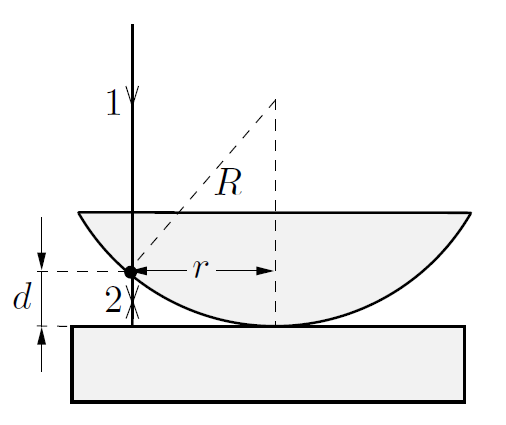
\includegraphics[scale=0.5]{rings}
		\end{wrapfigure}	
		Геометрическая разность хода между интерферирующими лучами
		равна удвоенной толщине воздушного зазора 2d в данном месте.
		Для точки на сферической поверхности, находящейся на расстоянии $r$ от оси системы, имеем $r_2 
		= R_2 - 
		(R - d)^2 
		= 2Rd -
		 d_2$,
		где $R$ - радиус кривизны сферической поверхности.
		
		При $R \gg d$ получим $d = r_2/2R$. С учётом изменения фазы на $\pi$ при отражении
		волны от оптически более плотной среды
		(на границе воздух-стекло) получим \textit{оптическую разность хода} интерферирующих лучей:
		\begin{equation}
		\triangle = 2d + \dfrac{\lambda}{2} = \dfrac{r^2}{R} + \dfrac{\lambda}{2}.
		\end{equation}
		
		Радиусы темных колец: $r_m = \sqrt{m\lambda R}$, светлых: $r_m' = \sqrt{(2m-1)\lambda R/2}$
		
		\subparagraph{Экспериментальная установка}
		
		Для протяжённого источника линии равной толщины локализованы
		на поверхности линзы, если пластинка лежит на линзе, и вблизи по-
		верхности линзы, если линза лежит на пластинке, как в нашем случае.
		Наблюдение ведётся в отражённом свете.
		
		
		
			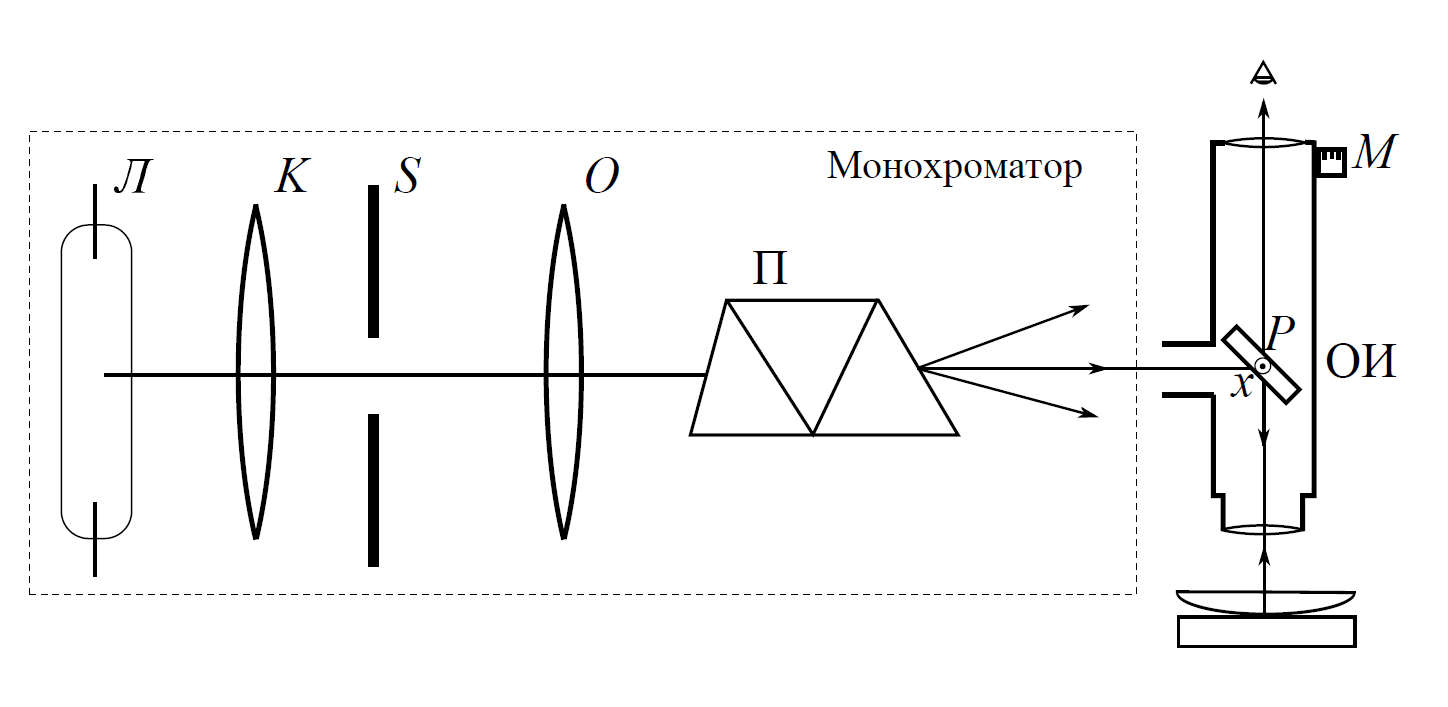
\includegraphics[scale = 0.5]{equipment}
		
		Источником света служит ртутная лампа, находящаяся в защитном кожухе. Для получения монохроматического света применяется	призменный монохроматор, состоящий из конденсора K, коллимато-
		ра (щель S и объектив O) и призмы прямого зрения П. Эти устройcтва с помощью рейтеров располагаются на оптической скамье. Свет от
		монохроматора попадает на опак-иллюминатор (ОИ), расположенный
		между окуляром и объективом микроскопа - специальное устройство
		для освещения объекта при работе в отражённом свете. Внутри опак-иллюминатора находится полупрозрачная пластинка P, наклоненная
		под углом $45^\circ$ к оптической оси микроскопа. Свет частично отражается от этой пластинки, проходит через объектив микроскопа и попадает
		на исследуемый объект. Пластинка может поворачиваться вокруг горизонтальной оси x, а опак-иллюминатор - вокруг вертикальной оси.
		
		
		\subparagraph{Определение радиуса кривизны}
		Для определения радиуса кривизны линзы измеряют диаметры колец: устанавливают перекрестие на середину какого-либо достаточно удалённого от центра, но ещё
		отчётливо видимого тёмного кольца и снимают отсчёт по окулярной
		шкале: целые деления отсчитываются слева от риски, проходящей через окулярную шкалу, десятые и сотые доли деления - по окулярному
		микрометрическому винту M.
		Перемещая перекрестие, последовательно устанавливают его на середины тёмных колец и записывают соответствующие показания окулярной шкалы и микрометра. После прохождения через центральное
		пятно продолжают измерения, записывая возрастающие номера колец
		и координаты их диаметров. Для устранения ошибок, возникающих из-за люфта в винте, перекрестие всегда следует подводить к кольцу с одной стороны. Цену одного деления окулярной шкалы определяют сравнивая её с изображением эталонной (объектной) шкалы. По разности
		отсчётов определяют диаметры, а затем и радиусы тёмных колец. Аналогичная серия измерений выполняется для светлых колец Ньютона.
		
		\subparagraph{Наблюдение биений}
		При освещении системы светом, содержащим две спектральные компоненты, наблюдается характерная картина
		биений: чёткость интерференционных колец периодически изменяется.
		Это объясняется наложением двух систем интерференционных колец,
		возникающих для разных длин волн $\lambda_1$ и $\lambda_2$. Чёткие кольца в результирующей картине образуются при наложении светлых колец на светлые и тёмных на тёмные. Размытые кольца получаются при наложении
		светлых колец одной картины на тёмные кольца другой.
		Нетрудно рассчитать период возникающих биений. Пусть в проме-
		жутке между двумя центрами соседних чётких участков укладывается
		m колец для спектральной линии с длиной волны $\lambda_1$. Тогда в этом
		промежутке должно располагаться ($\triangle m + 1$) колец для спектральной
		линии с длиной волны $\lambda_2$ (при $\lambda_2 < \lambda_1$).
		Для освещения входного окна опак-иллюминатора сразу двумя спектральными линиями (например, жёлтой и зелёной) можно
		расфокусировать монохроматор, смещая объектив O и призму.
		Если смешать две линии не удаётся, то, убрав призму прямого зрения, можно объективом O сфокусировать на окно опак-иллюминатора
		белый свет ртутной лампы. Результаты измерений не изменятся, так
		как остальные линии в спектре ртутной лампы заметно слабее жёлтой
		и зелёной.
		
		\paragraph{Обработка результатов}
		
		\subparagraph{Определение радиуса кривизны}
		
		
		Теория говорит (см. раздел "Кольца Ньютона"), что радиусы темных и светлых колец, полученных в результате интерференции, равны соответственно $r_m = \sqrt{m\lambda R}$
		 и $r_m' = \sqrt{(2m-1)\lambda R/2}$. Возведя данные равенства в квадрат, получим формулу для радиуса кривизны линзы. При этом радиус кривизны будет равен величине коэффициенту наклона прямой, выражающей зависимость $r_m^2/\lambda (m)$. Построим эти графики (с учетом калибровки, проведенной в конце работы, 1 деление шкалы микроскопа примерно равняется $0,100\pm 0,001$ мм).
		
		\begin{center}
		\captionof{table}{Подсчет радиусов темных колец}
		\begin{tabular}{|c|c|c|c|c|}
			\hline 
			№ & левый край, дел. шкалы & правый край, дел. шкалы & $d$, дел. шкалы  & $r_m$, мм \\ 
			\hline 
			1 & 2,42 & 4,8 & 2,38 & 0,119 \\ 
			\hline 
			2 & 2,04 & 5,34 & 3,3 & 0,165 \\ 
			\hline 
			3 & 1,7 & 5,78 & 4,06 & 0,203 \\ 
			\hline 
			4 & 1,49 & 6,11 & 4,62 & 0,231 \\ 
			\hline 
			5 & 1,22 & 6,45 & 5,23 & 0,2615 \\ 
			\hline 
		\end{tabular} 
	
		\captionof{table}{Подсчет радиусов светлых колец}
		\begin{tabular}{|c|c|c|c|c|}
			\hline 
			№ & левый край, дел. шкалы & правый край, дел. шкалы & $d$, дел. шкалы  & $r_m$, мм \\ 
			\hline 
			3 & 2,05 & 5,76 & 3,71 & 0,1885 \\ 
			\hline 
			4 & 1,71 & 6,12 & 4,41 & 0,2205 \\ 
			\hline 
			5 & 1,44 & 6,41 & 4,97 & 0,2485 \\ 
			\hline 
			6 & 1,22 & 6,72 & 5,5 & 0,275 \\ 
			\hline 
			7 & 0,99 & 6,98 & 5,99 & 0,2995 \\ 
			\hline 
			8 & 0,78 & 7,15 & 6,37 & 0,3185 \\
			\hline
		\end{tabular} 
		\end{center}
		
		По полученным данным построим графики зависимости $\dfrac{r_m^2}{\lambda} = f(m)$.
		
		
		\begin{minipage}{.6\textwidth}
			\centering
			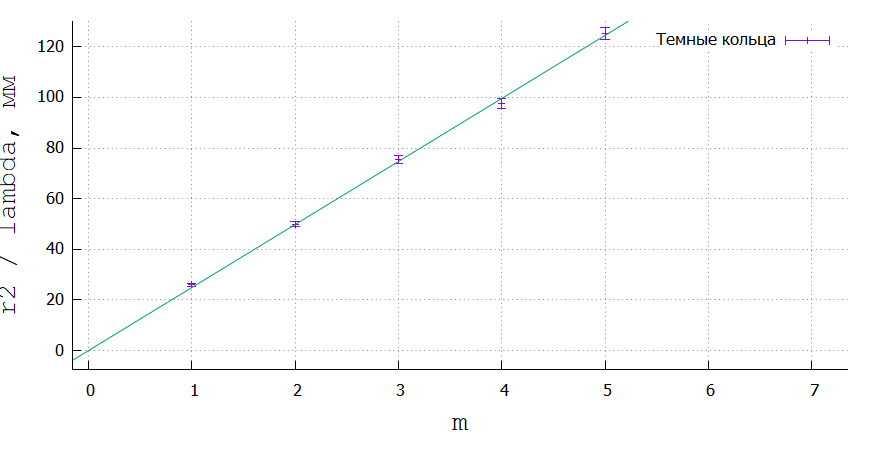
\includegraphics[scale=.6]{dark_plot}
			\captionof{figure}{График зависимости $\dfrac{r_m^2}{\lambda} = f(m)$ для темных колец}
		\end{minipage}	
		\begin{minipage}{.3\textwidth}
			$y = ax$\\
			$a = \rho = (24,89 \pm 0,16)$ мм
		\end{minipage}
	
		\vspace{3cm}
		
		\begin{minipage}{.6\textwidth}
			\centering
			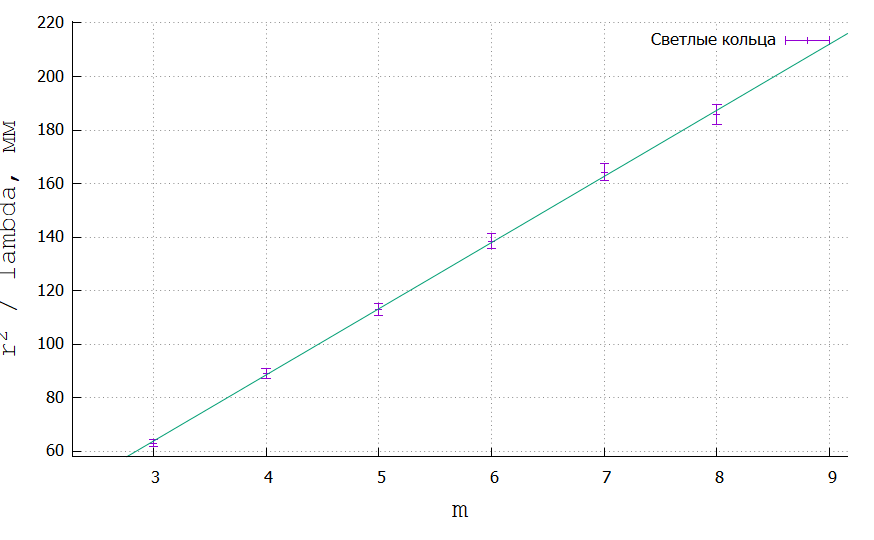
\includegraphics[scale=0.6]{light_plot}
			\captionof{figure}{График зависимости $\dfrac{r_m^2}{\lambda} = f(m)$ для светлых колец}
		\end{minipage}
		\begin{minipage}{.3\textwidth}
			$y = ax + b$\\
			$a = \rho = (25,05 \pm 0,26)$ мм
			$b = (-11,8 \pm 1,1)$ мм 
		\end{minipage}
		\vspace{2cm}
		
		В результате получили значение для радиуса кривизны $\boxed{\rho = (25,00\pm 0,26) mm}$.
		
		
		\subparagraph{Наблюдение биений}
		
		Найдем разность длин волн желтого и зеленого цвета по картине биений.
		
		При биениях мы имеем наложения $m$ минимума одной волны и $m+1$ минимума другой. Для радиусов темных колец имеем:
		\begin{equation}
			r_1 = \sqrt{mR\lambda_1},\;
			r_2 = \sqrt{(m-1)R\lambda_2}			
		\end{equation}
		
		Приравняв две величины, получим, что $$\Delta m = \dfrac{\lambda}{\Delta \lambda},$$ откуда
		\begin{equation}
		\Delta \lambda = \dfrac{\lambda}{\Delta m}
		\end{equation}
		
		В результате работы мы получили значение $m \simeq 13,5 \pm 0,5$. Тогда:
		$$\boxed{\Delta \lambda = 40,5 \pm 1,5}$$
		
		Значение для желтой волны - $586,5 \pm 1,5$ нм, что соответствует табличному значению (589 нм).
		
		\paragraph{Вывод}
		
		В ходе работы мы проделали классический опыт с получением колец Ньютона при нормальном падении света.
		Измерив диаметры темных и светлых колец и построив графики зависимостей, мы смогли определить радиус кривизны линзы, использовавшейся в работе. Также мы наблюдали картину биений. Оценив периодичность четких промежутков, мы смогли определить длину волны желтого цвета по длине волны зеленого цвета. Полученный результат сошелся с табличным.
	\end{document}
		